% ------------------------------------------------------------
% LaTeX Template für die DHBW zum Schnellstart!
% Original: https://github.wdf.sap.corp/D064996/LaTeX-Template-DHBW
% ------------------------------------------------------------
% ---- Präambel mit Angaben zum Dokument
\documentclass[
	fontsize=12pt,           % Leitlinien sprechen von Schriftgröße 12.
	paper=A4,
	twoside=false,
	listof=totoc,            % Tabellen- und Abbildungsverzeichnis ins Inhaltsverzeichnis
	bibliography=totoc,      % Literaturverzeichnis ins Inhaltsverzeichnis aufnehmen
	titlepage,               % Titlepage-Umgebung anstatt \maketitle
	headsepline,             % horizontale Linie unter Kolumnentitel
	abstracton,              % Überschrift einschalten, Abstract muss in {abstract}-Umgebung stehen
]{scrreprt}                  % Verwendung von KOMA-Report
\usepackage[utf8]{inputenc}  % UTF8 Encoding einschalten
\usepackage[ngerman]{babel}  % Neue deutsche Rechtschreibung
\usepackage[T1]{fontenc}     % Ausgabe von westeuropäischen Zeichen (auch Umlaute)
\usepackage{graphicx}        % Einbinden von Grafiken erlauben
\usepackage{wrapfig}         % Grafiken fließend im Text
\usepackage{setspace}        % Zeilenabstand \singlespacing, \onehalfspaceing, \doublespacing
\usepackage[
	%showframe,                % Ränder anzeigen lassen
	left=2.7cm, right=2.5cm,
	top=2.5cm,  bottom=2.5cm,
	includeheadfoot
]{geometry}                      % Seitenlayout einstellen
\usepackage{scrlayer-scrpage}    % Gestaltung von Fuß- und Kopfzeilen
\usepackage{acronym}             % Abkürzungen, Abkürzungsverzeichnis
\usepackage{titletoc}            % Anpassungen am Inhaltsverzeichnis
\contentsmargin{0.725cm}         % Abstand im Inhaltsverzeichnis zw. Punkt und Seitenzahl
\usepackage[                     % Klickbare Links (enth. auch "nameref", "url" Package)
  hidelinks,                     % Blende die "URL Boxen" aus.
  breaklinks=true                % Breche zu lange URLs am Zeilenende um
]{hyperref}
\urlstyle{same}                  % Aktuelle Schrift auch für URLs
% Anpassung von autoref für Gleichungen (ergänzt runde Klammern) und Algorithm
\addto\extrasngerman{%
	\def\equationautorefname~#1\null{Gleichung~(#1)\null}
	\def\lstnumberautorefname{Zeile}
	\def\algorithmautorefname{Algorithmus}
}

% ---- Abstand verkleinern von der Überschrift 
\renewcommand*{\chapterheadstartvskip}{\vspace*{.5\baselineskip}}

% ---- Für das Quellenverzeichnis
\usepackage[
	backend = biber,                % Verweis auf biber
	language = auto,
	style = numeric,                % Nummerierung der Quellen mit Zahlen
	sorting = none,                 % none = Sortierung nach der Erscheinung im Dokument
	sortcites = true,               % Sortiert die Quellen innerhalb eines cite-Befehls
	block = space,                  % Extra Leerzeichen zwischen Blocks
	hyperref = true,                % Links sind klickbar auch in der Quelle
	%backref = true,                % Referenz, auf den Text an die zitierte Stelle
	bibencoding = auto,
	giveninits = true,              % Vornamen werden abgekürzt
	doi=false,                      % DOI nicht anzeigen
	isbn=false,                     % ISBN nicht anzeigen
    alldates=short                  % Datum immer als DD.MM.YYYY anzeigen
]{biblatex}
\addbibresource{Inhalt/literatur.bib}
\setcounter{biburlnumpenalty}{3000}      % Umbruchgrenze für Zahlen
\setcounter{biburlucpenalty}{6000}       % Umbruchgrenze für Großbuchstaben
\setcounter{biburllcpenalty}{9000}       % Umbruchgrenze für Kleinbuchstaben
\DeclareNameAlias{default}{family-given}  % Nachname vor dem Vornamen
\AtBeginBibliography{
\renewcommand{\multinamedelim}{\addslash\space}
\renewcommand{\finalnamedelim}{\multinamedelim}
}  % Semikolon zwischen den Autorennamen
\DefineBibliographyStrings{german}{
  urlseen = {Einsichtnahme:},                      % Ändern des Titels von "besucht am"
}
\usepackage[babel,german=quotes]{csquotes}         % Deutsche Anführungszeichen + Zitate


% ---- Für Mathevorlage
\usepackage{amsmath}    % Erweiterung vom Mathe-Satz
\usepackage{amssymb}    % Lädt amsfonts und weitere Symbole
\usepackage{MnSymbol}   % Für Symbole, die in amssymb nicht enthalten sind.


% ---- Für Quellcodevorlage
\usepackage{scrhack}                    % Hack zur Verw. von listings in KOMA-Script
\usepackage{listings}                   % Darstellung von Quellcode
\usepackage{xcolor}                     % Einfache Verwendung von Farben
% -- Default Listing-Styles

\lstset{
	% Das Paket "listings" kann kein UTF-8. Deswegen werden hier 
	% die häufigsten Zeichen definiert (ä,ö,ü,...)
	literate=%
		{á}{{\'a}}1 {é}{{\'e}}1 {í}{{\'i}}1 {ó}{{\'o}}1 {ú}{{\'u}}1
		{Á}{{\'A}}1 {É}{{\'E}}1 {Í}{{\'I}}1 {Ó}{{\'O}}1 {Ú}{{\'U}}1
		{à}{{\`a}}1 {è}{{\`e}}1 {ì}{{\`i}}1 {ò}{{\`o}}1 {ù}{{\`u}}1
		{À}{{\`A}}1 {È}{{\'E}}1 {Ì}{{\`I}}1 {Ò}{{\`O}}1 {Ù}{{\`U}}1
		{ä}{{\"a}}1 {ë}{{\"e}}1 {ï}{{\"i}}1 {ö}{{\"o}}1 {ü}{{\"u}}1
		{Ä}{{\"A}}1 {Ë}{{\"E}}1 {Ï}{{\"I}}1 {Ö}{{\"O}}1 {Ü}{{\"U}}1
		{â}{{\^a}}1 {ê}{{\^e}}1 {î}{{\^i}}1 {ô}{{\^o}}1 {û}{{\^u}}1
		{Â}{{\^A}}1 {Ê}{{\^E}}1 {Î}{{\^I}}1 {Ô}{{\^O}}1 {Û}{{\^U}}1
		{œ}{{\oe}}1 {Œ}{{\OE}}1 {æ}{{\ae}}1 {Æ}{{\AE}}1 {ß}{{\ss}}1
		{ű}{{\H{u}}}1 {Ű}{{\H{U}}}1 {ő}{{\H{o}}}1 {Ő}{{\H{O}}}1
		{ç}{{\c c}}1 {Ç}{{\c C}}1 {ø}{{\o}}1 {å}{{\r a}}1 {Å}{{\r A}}1
		{€}{{\euro}}1 {£}{{\pounds}}1 {«}{{\guillemotleft}}1
		{»}{{\guillemotright}}1 {ñ}{{\~n}}1 {Ñ}{{\~N}}1 {¿}{{?`}}1,
	breaklines=true,        % Breche lange Zeilen um 
	breakatwhitespace=true, % Wenn möglich, bei Leerzeichen umbrechen
	% Symbol für Zeilenumbruch einfügen
	prebreak=\raisebox{0ex}[0ex][0ex]{\ensuremath{\rhookswarrow}},
	postbreak=\raisebox{0ex}[0ex][0ex]{\ensuremath{\rcurvearrowse\space}},
	tabsize=4,                                 % Setze die Breite eines Tabs
	basicstyle=\ttfamily\small,                % Grundsätzlicher Schriftstyle
	columns=fixed,                             % Besseres Schriftbild
	numbers=left,                              % Nummerierung der Zeilen
	%frame=single,                             % Umrandung des Codes
	showstringspaces=false,                    % Keine Leerzeichen hervorheben
	keywordstyle=\color{blue},
	ndkeywordstyle=\bfseries\color{darkgray},
	identifierstyle=\color{black},
	commentstyle=\itshape\color{JavaGruen},   % Kommentare in eigener Farbe
	stringstyle=\color{JavaBlau},             % Strings in eigener Farbe,
	captionpos=b,                             % Bild*unter*schrift
	xleftmargin=5.0ex
}

% ---- Eigener JAVA-Style für den Quellcode
\definecolor{JavaLila}{rgb}{0.4,0.1,0.4}
\definecolor{JavaGruen}{rgb}{0.3,0.5,0.4}
\definecolor{JavaBlau}{rgb}{0.0,0.0,1.0}

\renewcommand{\ttdefault}{pcr}               % Schriftart, welche auch fett beinhaltet
\lstdefinestyle{EigenerJavaStyle}{
	language=Java,                             % Syntax Highlighting für Java
	%frame=single,                             % Umrandung des Codes
	frame=lr,
	keywordstyle=\bfseries\color{JavaLila},    % Keywords in eigener Farbe und fett
	commentstyle=\itshape\color{JavaGruen},    % Kommentare in eigener Farbe und italic
	stringstyle=\color{JavaBlau}               % Strings in eigener Farbe
}

% ---- Eigener ABAP-Style für den Quellcode
\definecolor{ABAPKeywordsBlue}{HTML}{6000ff}
\definecolor{ABAPCommentGrey}{HTML}{808080}
\definecolor{ABAPStringGreen}{HTML}{4da619}

\renewcommand{\ttdefault}{pcr}
\lstdefinestyle{EigenerABAPStyle}{
	language=[R/3 6.10]ABAP,
	frame=lr,
	morestring=[b]\|,                          % Für Pipe-Strings
	morestring=[b]\`,                          % für Backtick-Strings
	keywordstyle=\bfseries\color{ABAPKeywordsBlue},
	commentstyle=\itshape\color{ABAPCommentGrey},
	stringstyle=\color{ABAPStringGreen},
	tabsize=2
}

% ---- Eigener Python-Style für den Quellcode
\definecolor{PyKeywordsBlue}{HTML}{0000AC}
\definecolor{PyCommentGrey}{HTML}{808080}
\definecolor{PyStringGreen}{HTML}{008080}

\renewcommand{\ttdefault}{pcr}
\lstdefinestyle{EigenerPythonStyle}{
	language=Python,
	columns=flexible,
	frame=lr,
	keywordstyle=\bfseries\color{PyKeywordsBlue},
	commentstyle=\itshape\color{PyCommentGrey},
	stringstyle=\color{PyStringGreen}
}

% ---- Eigener C#-Style für den Quellcode
\definecolor{CSharpKeywordsBlue}{HTML}{6000ff}
\definecolor{CSharpCommentGreen}{HTML}{4da619}
\definecolor{CSharpStringRed}{HTML}{aa2200}

\renewcommand{\ttdefault}{pcr}
\lstdefinestyle{EigenerCSharpStyle}{
	language=[Sharp]C,
	columns=flexible,
	frame=lr,
	rulecolor=\color{blue!80!black},
	keywordstyle=\bfseries\color{CSharpKeywordsBlue},
	commentstyle=\itshape\color{CSharpCommentGreen},
	stringstyle=\color{CSharpStringRed},
	morekeywords={dynamic}
}

% ---- Eigener C#-Style für den Quellcode
\definecolor{lightgray}{rgb}{.9,.9,.9}
\definecolor{darkgray}{rgb}{.4,.4,.4}
\definecolor{purple}{rgb}{0.65, 0.12, 0.82}

\renewcommand{\ttdefault}{pcr}
\lstdefinestyle{EigenerJavaScriptStyle}{
	frame=lr,
	keywords={typeof, new, true, false, catch, function, return, null, catch, switch, var, if, in, while, do, else, case, break},
	keywordstyle=\color{blue}\bfseries,
	ndkeywords={class, export, boolean, throw, implements, import, this},
	ndkeywordstyle=\color{darkgray}\bfseries,
	identifierstyle=\color{black},
	sensitive=false,
	comment=[l]{//},
	morecomment=[s]{/*}{*/},
	commentstyle=\color{purple}\ttfamily,
	stringstyle=\color{red}\ttfamily,
	morestring=[b]',
	morestring=[b]"
}  % Weitere Details sind ausgelagert

\usepackage{algorithm}                  % Für Algorithmen-Umgebung (ähnlich wie lstlistings Umgebung)
\usepackage{algpseudocode}              % Für Pseudocode. Füge "[noend]" hinzu, wenn du kein "endif",
                                        % etc. haben willst.

% ---- Tabellen
\usepackage{booktabs}  % Für schönere Tabellen. Enthält neue Befehle wie \midrule
\usepackage{multirow}  % Mehrzeilige Tabellen
\usepackage{siunitx}   % Für SI Einheiten und das Ausrichten Nachkommastellen
\sisetup{locale=DE, output-decimal-marker={,}} % Damit ein Komma und kein Punkt verwendet wird.

% ---- Für Definitionsboxen in der Einleitung
\usepackage{amsthm}                     % Liefert die Grundlagen für Theoreme
\usepackage[framemethod=tikz]{mdframed} % Boxen für die Umrandung
% ---- Definition für Highlight Boxen

% ---- Grundsätzliche Definition zum Style
\newtheoremstyle{defi}
  {\topsep}         % Abstand oben
  {\topsep}         % Abstand unten
  {\normalfont}     % Schrift des Bodys
  {0pt}             % Einschub der ersten Zeile
  {\bfseries}       % Darstellung von der Schrift in der Überschrift
  {:}               % Trennzeichen zwischen Überschrift und Body
  {.5em}            % Abstand nach dem Trennzeichen zum Body Text
  {\thmname{#3}}    % Name in eckigen Klammern
\theoremstyle{defi}

% ------ Definition zum Strich vor eines Texts
\newmdtheoremenv[
  hidealllines = true,       % Rahmen komplett ausblenden
  leftline = true,           % Linie links einschalten
  innertopmargin = 0pt,      % Abstand oben
  innerbottommargin = 4pt,   % Abstand unten
  innerrightmargin = 0pt,    % Abstand rechts
  linewidth = 3pt,           % Linienbreite
  linecolor = gray!40,       % Linienfarbe
]{defStrich}{Definition}     % Name der des formats "defStrich"

% ------ Definition zum Eck-Kasten um einen Text
\newmdtheoremenv[
  hidealllines = true,
  innertopmargin = 6pt,
  linecolor = gray!40,
  singleextra={              % Eck-Markierungen für die Definition
    \draw[line width=3pt,gray!50,line cap=rect] (O|-P) -- +(1cm,0pt);
    \draw[line width=3pt,gray!50,line cap=rect] (O|-P) -- +(0pt,-1cm);
    \draw[line width=3pt,gray!50,line cap=rect] (O-|P) -- +(-1cm,0pt);
    \draw[line width=3pt,gray!50,line cap=rect] (O-|P) -- +(0pt,1cm);
  }
]{defEckKasten}{Definition}  % Name der des formats "defEckKasten"  % Weitere Details sind ausgelagert

% ---- Eigene Packages von Felix Hausberger
%\usepackage{textcomp}
\usepackage{subfigure}
\usepackage{rotating}
\usepackage{setspace}
\usepackage[subfigure]{tocloft}
\usepackage{caption}

% ---- Für das Formelverzeichnis von Felix Hausberger
\newcommand{\listequationsname}{Formelverzeichnis}
\newlistof{equations}{equ}{\listequationsname}
\newcommand{\equations}[1]{%
\addcontentsline{equ}{equations}{\protect\numberline{\theequation}#1}\par}

% ---- Elektronische Version oder Gedruckte Version?
% ---- Unterschied: Die elektronische Version enthält keinen Platzhalter für die Unterschrift
\usepackage{ifthen}
\newboolean{e-Abgabe}
\setboolean{e-Abgabe}{true}    % false=gedruckte Fassung

% ---- Persönlichen Daten:
\newcommand{\titel}{Machbarkeitsstudie: Smart Warehouse}
\newcommand{\subtitel}{Echtzeit-Objektdetektoren im Vergleich}
\newcommand{\titelheader}{Deep Learning}
\newcommand{\arbeit}{Studienarbeit}
\newcommand{\studiengang}{Angewandte Informatik}
\newcommand{\studienjahr}{2019}
\newcommand{\autor}{Felix Hausberger und Robin Kuck}
\newcommand{\autorReverse}{Hausberger, Felix und Kuck, Robin}
\newcommand{\verfassungsort}{Karlsruhe}
\newcommand{\matrikelnr}{2773463, 4409176}
\newcommand{\kurs}{TINF17B2}
\newcommand{\bearbeitungsmonat}{Oktober 2019 - Mai 2019}
\newcommand{\abgabe}{18. Mai 2020}
\newcommand{\bearbeitungszeitraum}{30.09.2019 - 18.05.2020}
\newcommand{\firmaName}{SAP SE}
\newcommand{\firmaStrasse}{Dietmar-Hopp-Allee 16}
\newcommand{\firmaPlz}{69190 Walldorf, Deutschland}
\newcommand{\betreuerFirma}{}
\newcommand{\betreuerDhbw}{PD Dr.-Ing. Markus Reischl}

% ---- Metainformation für das PDF Dokument
\hypersetup{
	pdftitle    = {\titel},
	pdfsubject  = {\arbeit},
	pdfauthor   = {\autor},
	%pdfkeywords = {Keywords angeben},
	pdfcreator  = {LaTeX},
	%pdfproducer = {in der Regel pdfTeX}
}

% ---- Definition der Kopf- und Fußzeilen
\clearscrheadfoot                               % Löschen von LaTeX Standard
\automark[section]{chapter}                     % Füllen von section und chapter
\renewcommand*{\chaptermarkformat}{}            % Entfernt die Kapitelnummer
\renewcommand*{\sectionmarkformat}{}            % Entfernt die Sectionnummer
% Angaben [für "plain"]{für "scrheadings"}
\ihead[]{\titelheader}                          % Kopfzeile links
\chead[]{}                                      % Kopfzeile mitte
\ohead[]{\rightmark}                            % Kopfzeile rechts
\ifoot[]{}                                      % Fußzeile links
\cfoot*{\sffamily\pagemark}                     % Fußzeile mitte
\ofoot[]{}                                      % Fußzeile rechts
\KOMAoptions{
   headsepline = 0.2pt,                         % Liniendicke Kopfzeile
   footsepline = false                          % Liniendicke Fußzeile
}

% ---- Hilfreiches
\newcommand{\zB}{z.\,B. }   % "z.B." mit kleinem Leeraum dazwischen (ohne wäre nicht korrekt)
\newcommand{\dash}{d.\,h. }

% ---- Silbentrennung (falls LaTeX defaults falsch / nicht gewünscht sind)
\hyphenation{HANA}         % anstatt HA-NA
\hyphenation{Graph-Script} % anstatt GraphS-cript

% ---- Beginn des Dokuments
\begin{document}
\setlength{\parindent}{0pt}              % Keine Paragraphen Einrückung.
                                         % Dafür haben wir den Abstand zwischen den Paragraphen.
\setcounter{secnumdepth}{2}              % Nummerierungstiefe fürs Inhaltsverzeichnis
\setcounter{tocdepth}{1}                 % Tiefe des Inhaltsverzeichnisses. Ggf. so anpassen,
                                         % dass das Verzeichnis auf eine Seite passt.
\sffamily                                % Serifenlose Schrift verwenden.

% ---- Vorspann
% ------ Titelseite
\singlespacing
\thispagestyle{empty}
\begin{titlepage}
\enlargethispage{4cm}

\begin{figure}                    % Logo vom Ausbildungsbetrieb und der DHBW
	\begin{minipage}{0.49\textwidth}
		\flushleft
		
\includegraphics[height=2.5cm]{Bilder/Logos/Logo_SAP.pdf} 
	\end{minipage}
	\hfill
	\begin{minipage}{0.49\textwidth}
		\flushright
		
\includegraphics[height=2.5cm]{Bilder/Logos/Logo_DHBW.pdf} 
	\end{minipage}
\end{figure} 
\vspace*{0.1cm}

\begin{center}
	\huge{\textbf{\titel}}\\[1.5cm]
	\Large{\textbf{\subtitel}}\\[0.5cm]
	\Large{\textbf{\arbeit}}\\[0.5cm]
	\normalsize{im Rahmen der Prüfung zum\\[1ex] \textbf{Bachelor of Science (B.Sc.)}}\\[0.5cm]
	\Large{des Studienganges \studiengang}\\[1ex]
	\normalsize{an der Dualen Hochschule Baden-Württemberg Karlsruhe}\\[1cm]
	\normalsize{von}\\[1ex] \Large{\textbf{\autor}} \\[1cm]
	\normalsize{\bearbeitungsmonat}\\[1ex] \Large{\textbf{-Sperrvermerk-}}\\[0.5cm]
\end{center}

\begin{center}
	\vfill
	\begin{tabular}{ll}
		Abgabedatum:                     & \abgabe \\[0.2cm]
		Bearbeitungszeitraum:            & \bearbeitungszeitraum \\[0.2cm]
		Matrikelnummer, Kurs:            & \matrikelnr , \kurs \\[0.2cm]
		Ausbildungsfirma:                & \firmaName \\
		                                 & \firmaStrasse \\
		                                 & \firmaPlz \\[0.2cm]
		Gutachter an der DHBW:           & \betreuerDhbw \\[0.2cm]
	\end{tabular} 
\end{center}
\end{titlepage}  % Titelseite
\newcounter{savepage}
\pagenumbering{Roman}                    % Römische Seitenzahlen
\onehalfspacing

% ------ Erklärung, Sperrvermerk, Abstact
\chapter*{Eidesstattliche Erklärung}
Ich versichere hiermit, dass ich meine \arbeit{} mit dem Thema:
\begin{quote}
	\textit{\titel}
\end{quote} 
gemäß § 5 der \enquote{Studien- und Prüfungsordnung DHBW Technik} vom 29. September 2017 selbstständig verfasst und keine anderen als die angegebenen Quellen und Hilfsmittel benutzt habe. Die Arbeit wurde bisher keiner anderen Prüfungsbehörde vorgelegt und auch nicht veröffentlicht.

\vspace{0.25cm}

Ich versichere zudem, dass die eingereichte elektronische Fassung mit der gedruckten Fassung übereinstimmt.

\vspace{1cm}

\verfassungsort, den \today \\[0.5cm]
\ifthenelse{\boolean{e-Abgabe}}
	{\underline{Gez. \autor}}
	{\makebox[6cm]{\hrulefill}}\\ 
\autorReverse

\renewcommand{\abstractname}{Abstract} % Veränderter Name für das Abstract
\begin{abstract}
\begin{addmargin}[1.5cm]{1.5cm}        % Erhöhte Ränder, für Abstract Look
\thispagestyle{plain}                  % Seitenzahl auf der Abstract Seite

\begin{center}
\small\textit{- English -}             % Angabe der Sprache für das Abstract
\end{center}

\vspace{0.25cm}
In this thesis the object detectors \textit{You Only Look Once} and \textit{Single Shot MultiBox Detector} are compared for precision, reactivity, training and inference behaviour and examined for their potential for industrial use. The background scenario of the \textit{Smart Warehouse} offers live video data of a drone with goods in a warehouse, which are to be classified and localized in real time. In the future, this should make it possible to carry out inventories and inventory analyses of a warehouse in a time- and cost-efficient manner conserving resources.

\vspace{0.25cm}
The goal of this feasibility study is to find out whether the \textit{Smart Warehouse} scenario is technically feasible. In addition, the focus is also on the object detectors themselves, their differences in architecture and behavior and whether they are generally suitable for industrial application scenarios.

\end{addmargin}
\end{abstract}
\renewcommand{\abstractname}{Abstract} % Veränderter Name für das Abstract
\begin{abstract}
\begin{addmargin}[1.5cm]{1.5cm}        % Erhöhte Ränder, für Abstract Look
\thispagestyle{plain}                  % Seitenzahl auf der Abstract Seite

\begin{center}
\small\textit{- Deutsch -}             % Angabe der Sprache für das Abstract
\end{center}

\vspace{0.25cm}
Kurzbeschreibung

\end{addmargin}
\end{abstract}

% ------ Inhaltsverzeichnis
\singlespacing
\tableofcontents

% ------ Verzeichnisse
\renewcommand*{\chapterpagestyle}{plain}
\pagestyle{plain}
\setlength{\cftsecnumwidth}{3em}
\setlength{\cfttabnumwidth}{3em}            
%\chapter*{Formelverzeichnis}
\addcontentsline{toc}{chapter}{Formelverzeichnis} % Hinzufügen zum Inhaltsverzeichnis 

% Definition des neuen Befehls für das Einfügen der Abkürzung der Einheit
\newcommand{\acrounit}[1]{
  \acroextra{\makebox[18mm][l]{\si[per=frac,fraction=nice]{#1}}}
}
\begin{acronym}[dmin] % längstes Kürzel wird verw. für den Abstand zw. Kürzel u. Text

	%Lateinische
	%	Bezeichnungen erscheinen vor den griechischen Abkürzungen, die keine Formelzeichen darstellen, sind
	%	getrennt aufzuführen und außerdem beim ersten Gebrauch einzuführen.

	%Wichtige Formeln werden jeweils bei ihrem ersten Auftreten durch eingeklammerte Zahlen am Ende oder
	%Anfang der Zeile gekennzeichnet. Die gewählte Kennzeichnung ist in der gesamten Arbeit einheitlich beizubehalten.

	% Alphabetisch selbst sortieren - nicht verwendete Formeln rausnehmen!
	% Allgemein: \acro{KÜRZEL}[ABKÜRZUNG]{\acrounit{SI-EINHEIT}BESCHREIBUNG}

\end{acronym}
\chapter*{Abkürzungsverzeichnis}
\addcontentsline{toc}{chapter}{Abkürzungsverzeichnis} % Hinzufügen zum Inhaltsverzeichnis 

\begin{acronym}[WYSISWG] % längstes Kürzel wird verw. für den Abstand zw. Kürzel u. Text

	% Alphabetisch selbst sortieren - nicht verwendete Kürzel rausnehmen!
	% Keine Umgangssprachlichen Abkürzungen
	%Lateinisch vor griechisch
	
	\acro{AI}{Artificial Intelligence}
	\acro{ANN}{Artificial Neural Network}
	\acro{ASIC}{Application-Specific Integrated Circuit}
	\acro{AWS}{Amazon Web Services}
	\acro{CNN}{Convolutional Neural Network}
	\acro{COCO}{Common Objects in Context}
	\acro{CLI}{Command Line Interface}
	\acro{CPU}{Central Processing Unit}
	\acro{CUDA}{Compute Unified Device Architecture}
	\acro{DBN}{Deep Belief Network}
	\acro{DevOps}{Development Operations}
	\acro{DLL}{Dynamic Link Library}
	\acro{EASA}{European Aviation Safety Agency}
	\acro{ELU}{Exponential Linear Unit}
	\acro{FCN}{Fully Convolutional Network}
	\acro{FLOPS}{Floating Point Operations Per Second}
	\acro{FPGA}{Field Programmable Gate Array}
	\acro{FPS}{Frames Per Second}
	\acro{GCP}{Google Cloud Platform}
	\acro{GPU}{Graphics Processing Unit}
	\acro{IoU}{Intersection over Union}
	\acro{LReLU}{Leaky Rectified Linear Unit}
	\acro{MLP}{Multi-Layer Perzeptron}
	\acro{mAP}{mean Average Precision}
	\acro{PReLU}{Parametric Rectified Linear Unit}
	\acro{PascalVOC}{Pascal Visual Object Classes}
	\acro{PaaS}{Platform-as-a-Service}
	\acro{R-CNN}{Regional Convolutional Neural Network}
	\acro{ReLU}{Rectified Linear Unit}
	\acro{REST}{Representational State Transfer}
	\acro{RoI}{Region of Interest}
	\acro{RPN}{Region Proposal Network}
	\acro{SaaS}{Software-as-a-Service}
	\acro{SDK}{Software Development Kit}
	\acro{SSD}{Single Shot MultiBox Detector}
	\acro{TOPS}{Tera Operations Per Second}
	\acro{TPU}{Tensor Processing Unit}
	\acro{XML}{Extensible Markup Language}
	\acro{YOLO}{You Only Look Once}

\end{acronym}
\addcontentsline{toc}{chapter}{Abbildungsverzeichnis}
\listoffigures
\setlength{\cftequationsnumwidth}{2,5em}
\setlength{\cftequationsindent}{\cfttabindent}
\addcontentsline{toc}{chapter}{Formelverzeichnis}
\listofequations 
%\listoftables                           % Erzeugen des Tabellenverzeichnisses
\renewcommand{\lstlistlistingname}{Listenverzeichnis}
\lstlistoflistings                      % Erzeugen des Listenverzeichnisses
\setcounter{savepage}{\value{page}}


% ---- Inhalt der Arbeit
\cleardoublepage
\pagenumbering{arabic}                  % Arabische Seitenzahlen für den Hauptteil
\setlength{\parskip}{0.5\baselineskip}  % Abstand zwischen Absätzen
\rmfamily
\renewcommand*{\chapterpagestyle}{scrheadings}
\pagestyle{scrheadings}
\onehalfspacing
\setcounter{chapter}{-1}
\chapter{Vorwort}

Besonderen Dank ist an unseren Betreuer PD Dr. -Ing. Markus Reischl auszusprechen, ohne den die folgenden Forschungsergebnisse nicht zustande gekommen wären. Auch dem Informatik Labor unter Enrico Hühneborg der DHBW ist für die nötige finanzielle Unterstützung zum Erwerb der Drohne zu danken.

\chapter{Grundlagen und Forschungsstand}

Neben einer Einführung in den Anwendungsbereich von \textit{Deep Learning} zur Bildverarbeitung soll sich das folgende Kapitel speziell mit Architekturen unterschiedlicher Objektdetektoren auseinander setzen und herausstellen, wie sich diese voneinander abgrenzen. Davor wird allerdings zunächst grundlegendes Wissen über neuronale Netze und wie diese \glqq lernen\grqq{} vermittelt sowie wie ein eigener Datensatz zu gestalten ist. Abschließend werden technische Grundlagen für die Programmierung des \textit{Smart Warehouse} Szenarios aufgezeigt.

\section{Deep Learning zur Bildverarbeitung}

Ein klassisches Anwendungsgebiet von \textit{Deep Learning} zu Bildverarbeitung oder auch allgemein von maschinellem Lernen beschreibt die \textit{Klassifikation}. Hierbei werden bestimmte Kategorien, auch \textit{Klassen} genannt, definiert, in die ein Bild eingeordnet werden soll. Die \textit{Klassifikation} wird anhand von aus dem Bild extrahierten Merkmalen, auch \textit{Features} genannt, getroffen. Die Merkmale werden zu einem \textit{Merkmalsvektor} oder auch \textit{Feature Map} zusammengefasst und von einem \textit{neuronalen Netz} verarbeitet. Das Ergebnis der Verarbeitung durch das neuronale Netz ist die Einordnung in eine bestimme Klasse. 

Zusätzlich zur \textit{Klassifikation} eines Bildes kann das auf dem Bild abgebildete Objekt ebenfalls lokalisiert werden. Es wird dann von sogenannter \textit{Objektdetektion} gesprochen. Es können auch mehrere Objekte auf einem Bild detektiert werden. Ergebnis der Objektdetektion ist somit nicht nur eine Klasseneinordnung sondern ebenso eine klare Positionsangabe des Objektes auf dem Bild. Die Positionsangabe erfolgt durch Angabe sogenannter \textit{Bounding Boxen}. Diese umrahmen das jeweils detektierte Objekt und werden durch ihren linken oberen Eckpunkt sowie ihre Höhe und Breite beschrieben. 

Neben der klassischen \textit{Klassifikation} und der \textit{Objektdetektion} existiert ebenso ein drittes Anwendungsgebiet von \textit{Deep Learning} zu Bildverarbeitung, die \textit{Segmentierung}. Bei der \textit{semantischen Segmentierung} wird versucht, jede einzelne Pixel eines Bildes einer Klasse zuzuordnen und dementsprechend farblich im Bild zu hinterlegen. \textit{Instanzbasierte Segmentierung} hingegen zielt darauf ab, nicht nur jeden Pixel zu einer Klasse zu klassifizieren, sondern ebenso eine Identität zu einem Objekt zuzuweisen \cite{RavindraParmar.20180902}. Es setzt sich zusammen aus \textit{semantischer Segmentierung} und paralleler \textit{Objektdetektion}.

Einen Überblick über die vorgestellten Anwendungsgebiete ist in Abbildung \ref{applications} zu sehen.

\begin{figure}[ht]
	\begin{center}
		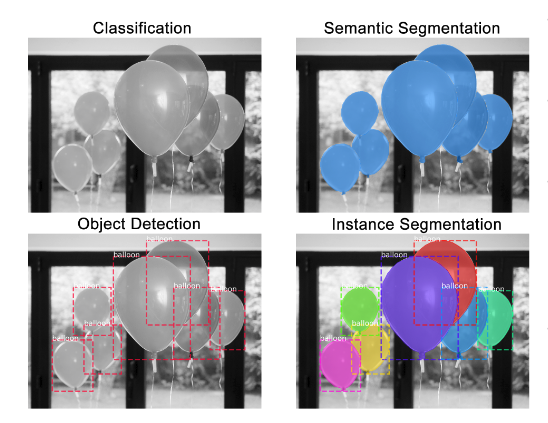
\includegraphics[width=12cm]{Bilder/applications.png} 
		\caption[Anwendungsgebiete von Deep Learning zur Bildverarbeitung im Überblick]{Anwendungsgebiete von Deep Learning zur Bildverarbeitung im Überblick \cite{PriyaDwivedi.20190328}}
		\label{applications}
	\end{center}
\end{figure}

Für eine einfache \textit{Klassifikation} eines Bildes können einfache sogenannte \textit{Feed-Forward} Netze verwendet werden. Es kann hierbei aber auch auf konventionelle Methoden der Bildverarbeitung zurück gegriffen werden. Für die \textit{Objektdetektion} stehen Architekturen wie \textit{You Only Loom Once} (YOLO), der \textit{Single Shot MultiBox Detector} (SSD) oder neuronale Netze der \textit{Regional Proposal Neural Networks} (R-CNN) bereit. Aus dieser Familie entstammt ebenso das \textit{Mask R-CNN} Netz, das zur \textit{Instanzbasierten Segmentierung} von Objekten verwendet wird.

\section{Problemstellung und Motivation}

Das \textit{Smart Warehouse} beschreibt ein Warenhaus, welches unter Einsatz einer Drohne in der Lage sei soll Inventuren und Bestandsprüfungen weitgehend ohne menschliche Hilfe durchzuführen. Das Live-Bild der Drohne soll von den Objektdetektoren dazu genutzt werden, Warengegenstände zu lokalisieren und klassifizieren. 

Neben der Frage, ob ein solches Industrieszenario überhaupt umsetzbar und wirtschaftlich sinnvoll ist, sollen die Objektdetektoren in diesem Anwendungsszenario nach verschiedenen Kriterien miteinander verglichen und beurteilt werden. Diese Kriterien lassen sich hauptsächlich in die Kategorien Präzision, Reaktionsvermögen und Trainingsverhalten untergliedern und werden später genauer eingeführt. Dadurch lassen sich Aussagen darüber treffen, ob nach dem momentanen Forschungsstand um Objektdetektoren solche das Potential bieten, industriell eingesetzt zu werden. 

Falls die Machbarkeitsstudie des \textit{Smart Warehouse} glückt, so kann der Industrie ein kostengünstiges, zeitsparendes und ressourcenschonendes Modell zur Inventurverwaltung eines Warenhauses angeboten werden.
\section{Vorgehensweise und Zielsetzung}

Im Grundlagenkapitel 2 muss sich mit den theoretischen Grundlagen von CNNs und Objektdetektoren auseinander gesetzt werden. Hierzu ist zunächst eine Einführung in Deep Learning zur Bildverarbeitung und neuronale Netz erforderlich, darunter zu Perzeptronen, dem Gradientenverfahren, dem Backpropagation Algorithmus und Hyperparametern zum Trainieren eines neuronalen Netzes (siehe Kapitel \ref{bildverarbeitung}, \ref{anns} und \ref{hyperparam}). 

Um weitere Grundlagen zum Training von neuronalen Netzen einzuführen, wird anschließend über die Anforderungen eines Datensatzes gesprochen (siehe Kapitel \ref{data}), bevor weitere Grundlagen zu Objektdetektoren eingeführt werden (siehe Kapitel \ref{basics}). 

Nachdem zu Beginn des Kapitels \ref{basics} kurz auf den Grundbaustein moderner Objektdetektoren eingegangen wird, den CNNs, können anschließend die Funktionsweisen und Architekturen der drei miteinander verglichenen Objektdetektoren der \textit{R-CNN} Familie, \textit{YOLO} und des \textit{SSDs} erläutert werden (siehe Kapitel \ref{detection}). Bei \textit{R-CNN} und \textit{YOLO} ist zu bemerken, dass unterschiedliche Evolutionsstufen der Detektoren zu betrachten sind.

Um weitere Grundlagen zum Training von neuronalen Netzen einzuführen, wird anschließend über zwei wesentlichen Speicherformate eines Datensatzes gesprochen (siehe Kapitel \ref{format}), bevor verschiedene Cloud Anbieter für das Trainieren von \textit{Deep Learning} Modellen aufgezeigt werden (siehe Kapitel \ref{cloud}). 

In Kapitel 3 werden chronologisch Teilziele der Konzeption beschrieben, darunter das Erstellen eines Trainingsdatensatzes (siehe Kapitel \ref{traindata}), dem Einführen von Bewertungskriterien (siehe Kapitel \ref{eval}), der Auswahl von Objektdetektoren, der Trainingsinfrastruktur und der Drohne (siehe Kapitel \ref{detect}, \ref{infrastructure}, \ref{drone_selection}) und die Spezifikation der Inventursoftware (siehe Kapitel \ref{software}).

In der Realisierung werden die Herausforderungen zur Steuerung und Anbindung der Drohne betrachtet und zudem die Objektdetektoren auf die realen Datensätze trainiert. Auch die Entwicklung der Webapplikation zur Visualisierung des Live-Bildes und der erkannten Objekte sowie der darin realisierte Zählalgorithmus zur Durchführung der Inventur wird Bestandteil dieses Kapitels sein. Die Ergebnisse der Realisierungsphase werden nach den in Unterkapitel \ref{eval} definierten Bewertungskriterien im folgenden Kapitel dargestellt. 

Ziel der Arbeit ist es Aussagen über die Fähigkeit von Objektdetektoren zum Einsatz in der Industrie zu treffen, indem eine Bewertung der Verhaltensweisen der Objektdetektoren nach den eingeführten Bewertungskriterien durchgeführt wird. Als Umgebung und Rahmenszenario für die Evaluation dient das \textit{SmartWarehouse} Szenario, dessen Machbarkeit ebenfalls herausgestellt werden soll (siehe Kapitel \ref{evaluation}).

Zuletzt wird das Wesen der Arbeit nochmals kurz zusammengefasst und anschließend auf mögliche Verbesserungen und Ausblicke in die Zukunft aufmerksam gemacht. 


\chapter{Stand der Technik}

\section{Neuronale Netze}


\section{Convolutional Neural Networks}


\section{Objektdetektoren}

\subsection{Regional Convolutional Neural Networks}

\subsection{You Only Look Once}

\subsection{Single Shot MultiBox Detector}

\section{Einsatz in der Industrie}

\section{PyTorch}

\begin{itemize}
	\item Methoden
	\item Literaturrecherche
	\item Herausarbeitung des Neuheitswertes 
\end{itemize}


\section{Einführen von Bewertungskriterien}

Um Objektdetektoren miteinander vergleichbar zu machen und um deren Potential zum industriellen Einsatz zu bewerten, müssen konkrete Bewertungskriterien eingeführt werden.

\subsection*{Präzision}

Zur Messung der Präzision wird die Metrik \textit{mAP} verwendet. Dies garantiert eine gute Vergleichbarkeit mit den veröffentlichten Leistungsmerkmalen der Objektdetektoren.

\subsection*{Reaktionsvermögen}

Um eine Verarbeitung in Echtzeit zu ermöglichen, muss gewährleistet sein, dass die Inferenzgeschwindigkeit mit dem Modell mit der eingehenden Bildrate einhergeht. Als Maßstab dafür dient die \textit{Frames Per Second} (FPS) Zahl. Echtzeitfähigkeit in der Machbarkeitsstudie ist so definiert, dass die Inferenz mit dem Modell mindestens so schnell ablaufen muss, dass Änderungen in der Umgebung rechtzeitig von Objektdetektor noch wahrgenommen werden können. 

\subsection*{Trainingsverhalten}

Unter dem Punkt Trainingsverhalten wird zusammengefasst, wie schnell sich die einzelnen Modelle mit den unterschiedlichen Objektdetektoren trainieren lassen. Hierbei wird besonderer Fokus darauf gelegt, wie viele Trainingsepochen notwendig sind, bis der Gradient der Fehlerfunktion des neuronalen Netzes keine merkenswerten Fortschritte auf Basis des verwendeten Datensatzes mehr erzielt.

\subsection*{Inferenzverhalten}

Im Zuge der Evaluation des Inferenzverhaltens werden vier Kriterien betrachtet. 

\begin{itemize}
	\item Das Verhalten bei besonderen Beleuchtungsverhältnissen wie unterbeleuchteten oder überbeleuchteten Gegenden.
	\item Das Verhalten bei extremen Blicklagen auf Basis der Entfernung und des Winkels zum detektierenden Objekt.
	\item Das Verhalten bei nicht vollständig sichtbaren Objekten, z.B. bei Verdeckung.
	\item Der Umgang mit doppelt detektierten Objekten. 
\end{itemize}

\section{Variantendiskussion mit Benchmarkdaten}

\begin{itemize}
	\item Verfahren incl. Variantendiskussionen
	\item Funktionsweise an Benchmarkdatensatz erklären
	\item Parameter d. Methode diskutieren und u.U. bestimmen
\end{itemize}

\section{Datensatz}

\begin{itemize}
	\item Richtigen Datensatz beschreiben
\end{itemize}

\chapter{Realisierung}

Im folgenden Abschnitt soll auf die Implementierung des \textit{Smart Warehouse} Szenarios eingegangen werden. Insbesondere werden Probleme während der Umsetzung der beiden Objektdetektoren \textit{SSD} und \textit{YOLO} betrachtet, die Realisierung der Dashboard-Webapplikation und des Zählalgorithmus zur Durchführung der Inventur aufgezeigt und letztendlich Herausforderungen im Rahmen der Drohnen Anbindung besprochen.

\section{Umsetzung der Objektdetektoren}

\subsection*{SSD}

Die verwendete Custom-Implementierung in \textit{PyTorch} realisiert die \textit{SSD300} Variante des \textit{SSDs}. Neben kleineren Änderungen in der Codebasis zur Erreichung von Kompatibilität mit aktuellen Bibliotheksversionen und weiteren Anpassungen zur Integration eines eigenen Datenbestandes, wurden vor allem drei größere Erweiterungen durchgeführt. 

Da der erstellte Datenbestand nur 1088 gelabelte Daten enthält, wurde zusätzlich zur Custom-Implementierung ein sechsfaches Kreuzvalidierungsverfahren realisiert. Es dient dazu ein höheres Abstraktionsvermögen des Modells auf dem geringen Datenbestand zu erreichen. Auch unterstützte die Referenzimplementierung keine Validierung durch zuvor ungesehene Daten. Die Modellklassen des Datenbestandes und die Validierungsskripte wurden dahingehend angepasst. Zudem fehlte eine Visualisierung der Entwicklung der Verlustkurven während des Trainingsverfahrens.

Die Referenzimplementierung erstellt sich des Weiteren einige Hilfsdateien, in der die Pfade zu Bildern und weitere Datenstrukturen für Trainingszwecke abgespeichert werden. Ohne diese ist kein Training möglich, das Trainingsskript fordert demnach Zugriff auf den Sekundärspeicher. 

Um ein lokales Training auf der \textit{NVIDIA GeForce GTX 1080} GPU zu ermöglichen, wurde zudem \textit{CUDA} Version 10.1 verwendet. Trainiert wurde mit folgenden Hyperparametern:
\begin{itemize}
	\item Batchgröße: 16
	\item Lernrate: $1.0\cdot 10^{-3}$
	\item Momentum: 0.9
	\item Kreuzvalidierungen: 6 à 22 Epochen
	\item Epochen: 132
	\item Gradientenverfahren: Stochastic Gradient Descent
	\item Kostenfunktion: Smooth L1
\end{itemize}

Das Basisnetzwerk des \textit{SSDs} besteht aus einem auf \textit{ImageNet} vortrainierten \textit{VGG16}. Die restlichen \textit{Convolutional Layer} sind \textit{Xavier} initialisiert. 

Die Hyperparameter sind nahezu gleich zu denen in der ursprünglichen wissenschaftlichen Veröffentlichung. Die Batch Größe im \textit{Mini-Batch} Verfahren wurde für größere Stabilität von 32 auf 16 heruntergesetzt. Auch in der Evaluierung wurde die Batch Größe von 64 auf 48 verkleinert, da die Eingangsdaten eine weitaus höhere Auflösung als die ursprünglich im \textit{PascalVOC} verwendeten Daten haben. Andernfalls wird Gefahr gelaufen, einen Speicherüberlauf zu verursachen. Der Datensatz wurde in fünf Untermengen unterteilt, in jedem Kreuzvalidierungsschritt diente jeweils eine Untermenge als Testdatensatz.

\subsection*{YOLO}

Für \textit{YOLO} wurde die neuste Version \textit{YOLOv3} implementiert. Hierbei kommt das \textit{Dark-""net} Framework zum Einsatz, eine Implementierung in C. Vor der initialen Kompilierung müssen einige Konfigurationsschritte unternommen werden, weil auch der Betrieb auf einer normalen CPU oder einer GPU mit Tensor Kernen möglich ist. Für das Training kommt eine \textit{NVIDIA GeForce RTX 2060 SUPER} GPU zum Einsatz, deren enthaltenen Tensor Kerne mitbenutzt werden. Die benötigten Hyperparameter wurden dabei wie folgt gesetzt:

\begin{itemize}
	\item Batchgröße: 64
	\item Subdivisions: 16
	\item Lernrate: $1.0\cdot 10^{-3}$
	\item Momentum: 0.9
	\item Maximale Anzahl Batches: 18000
\end{itemize}

Im Unterschied zum \textit{SSD} kann \textit{YOLO} die in den GPU Speicher zu ladende Datenmenge eines Batches durch sogenannte \textit{Subdivisions} festgelegt. Hierbei werden nur noch $Batchgroesse \div Subdivisions$ Bilder gleichzeitig in die GPU geladen, um einen Speicherüberlauf zu vermeiden.

Die Lernrate sowie das Momentum bleiben wie in der Dokumentation empfohlen unverändert zu den Referenzwerten. Im Gegensatz zu \textit{SSD} wird kein Maximum für die Anzahl an Epochen, sondern ein Maximalwert für die zu durchlaufenen Batches gesetzt. Dieser Wert wird abhängig von der Menge an gelabelten Klassen gesetzt und kann als Empfehlung aus der Dokumentation für das \textit{Darknet} Framework entnommen werden. 

\section{Dashboard Entwicklung}

Der Server wurde mit dem \textit{Flask} Framework in Python implementiert und läuft auf dem \textit{Web Server Gateway Interface} (WSGI) server \textit{Waitress}. Er führt den Inferenzalgorithmus des \textit{SSDs} bzw. des \textit{YOLO} Objektdetektors für jeden Frame des empfangenen Videostreams der Drohne aus und streamt die inferierten Bilder mit den Bounding Boxen an jeden Client. Der Client wurde mit dem \textit{Bootstrap} Framework grafisch gestaltet (siehe Abbildung \ref{webapp}).

\begin{figure}[H]
	\begin{center}
		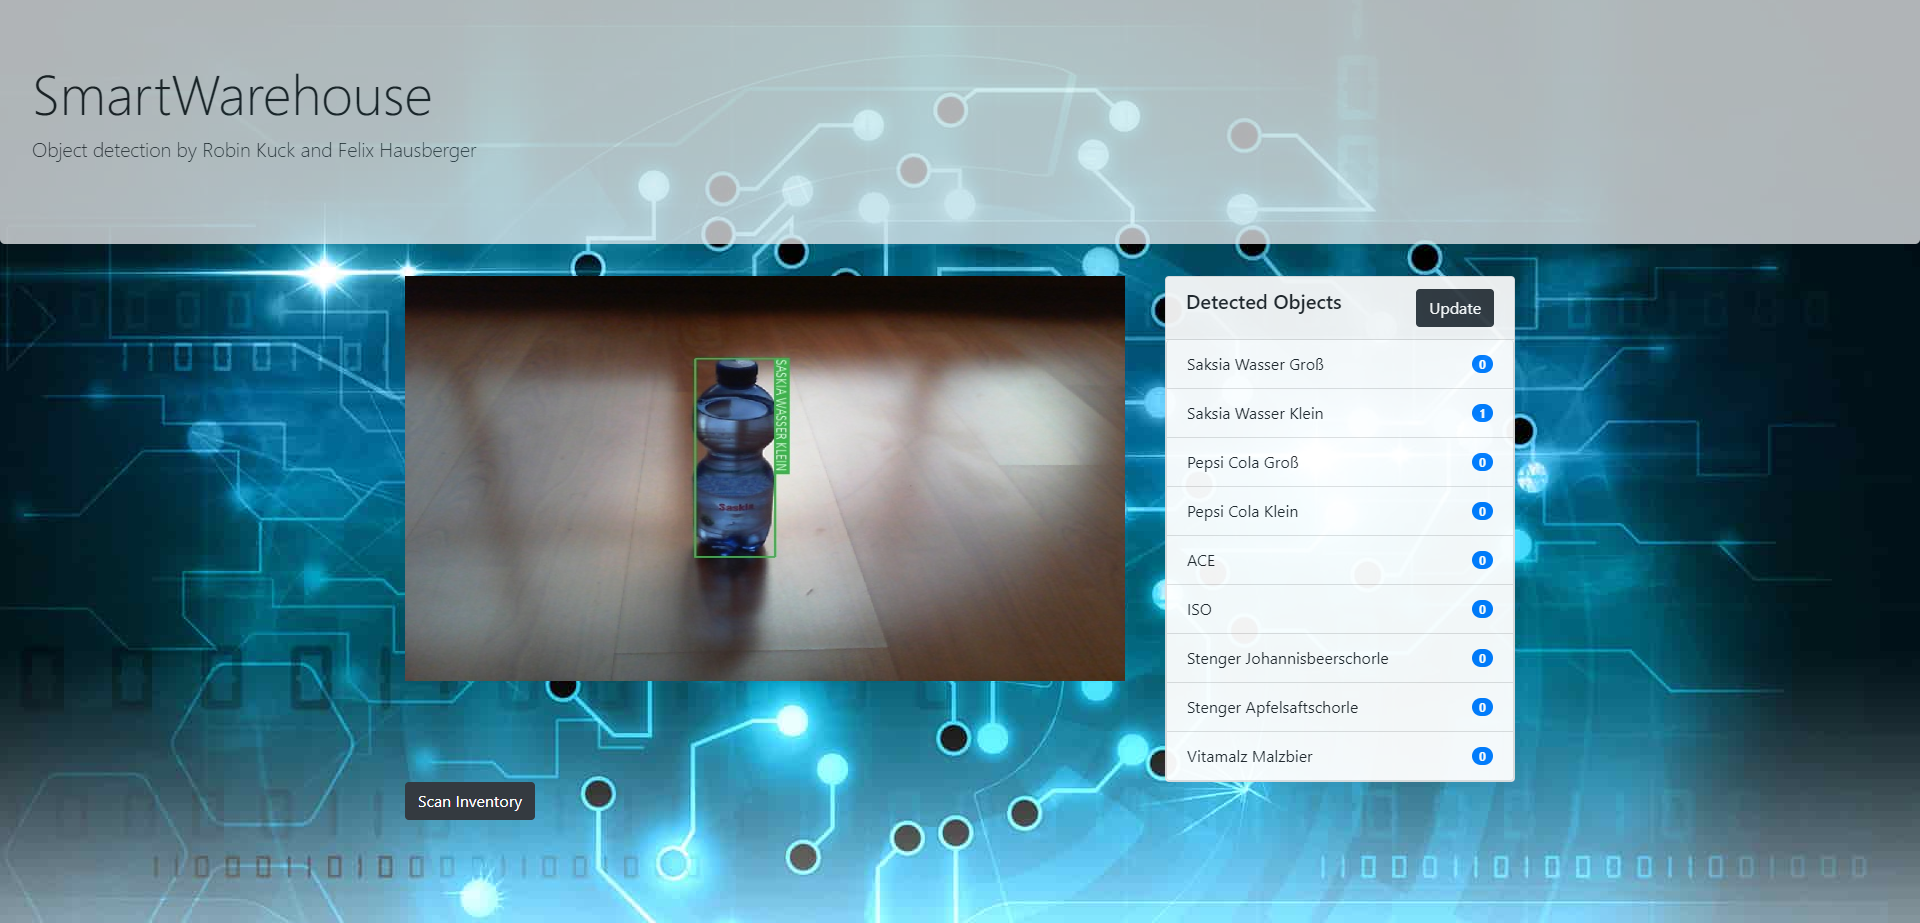
\includegraphics[width=15cm]{Bilder/webapp.jpeg} 
		\caption[Webapplikation SmartWarehouse]{Webapplikation SmartWarehouse}
		\label{webapp}
	\end{center}
\end{figure}

Auf Anfrage eines Client kann dieser die aktuell gezählten Objekte vom Server abfragen. Der Zählalgorithmus wird im folgenden Unterkapitel erklärt. 

\section{Zählalgorithmus}

\lstinputlisting[
label={code:formfield},
caption={Zählalgorithmus zum Zählen der detektierten Objekte},
captionpos=b,
basicstyle=\ttfamily\scriptsize,   
firstline=1,              
lastline=11                 
]{Quellcode/algorithmus.txt}

Der Algorithmus \ref{code:formfield} wird momentan dazu verwendet, um für das Industrieszenario einer Inventur einzelne detektierte Objekte zu zählen. Nach jedem Inferenzvorgang werden die detektierten Objekte abgespeichert, sodass der Algorithmus bei Aufruf sowohl auf die zuletzt detektierten Objekte \textit{o\_alt}, als auch auf die neu detektierten Objekte \textit{o\_neu} zugreifen kann. Für alle detektierten Objekte im aktuellen Durchlauf durchsucht er alle zuletzt detektierten Objekte, um herauszufinden, ob ein Objekt bereits im vorherigen Bild vorhanden war. Ausschlaggebend hierfür ist das gleiche \textit{Label} als auch die Distanz der Bounding Boxen des aktuell detektierten Objekts zum Objekt der Vorrunde. Nur falls das Objekt nach diesen Kriterien nicht bereits in der Vorrunde vorhanden war, wird es gezählt. Das Problem, das der Algorithmus zu lösen versucht, enthält allerdings eine weitere Komplexitätsstufe. Dasselbe Objekt kann im Laufe der Inventur erneut auftreten und dessen relative Position im Bild ist ebenso variabel. In diesem Falle werden Objekte doppelt gezählt. 

\section{Drohnen Anbindung}

\subsection*{Flugsequenz}
Wie in Kapitel \ref{drone_selection} beschrieben wird das Versenden von Befehlen mittels einer bidirektionalen Verbindung realisiert. Die Kommunikation durch eine Socket\footnote{Mit Sockets können Daten bidirektional zwischen  Programmen ausgetauscht werden, die entweder auf dem gleichen oder auf einem anderen durch eine Netzwerkadresse erreichbaren PC laufen.} Verbindung ist dabei eine passende Lösung. Python bietet ein \textit{socket} Modul an, welches verschiedene Typen von Sockets unterstützt. Das nachfolgende Listing zeigt die Initialisierung einer Instanz der Socket Klasse:

\lstinputlisting[
label={code:python},
caption={Initialisierung der Socket Klasse},
captionpos=b,
basicstyle=\ttfamily\scriptsize,   
firstline=1,              
lastline=2                 
]{Quellcode/socket_init.py}

Die Methode \textit{socket()} erzeugt eine neue Instanz der Socket Klasse und benötigt zwei Parameter für die Adressfamilie und den Verbindungstyp. \textit{AF\_INET} steht für Internet-Socket-Adresse, die sich aus IP-Adresse und Portnummer zusammensetzt. Der Parameter \textit{SOCK\_DGRAM} gibt an, dass die Socket Verbindung über das UDP-Protokoll aufgebaut wird. Für das Empfangen von Daten wird die Instanz zusätzlich an eine Adresse (hier \textit{localhost:9000}) gebunden.

Im folgenden Listing wird jeweils die Methode zum Senden von Befehlen und Empfangen von Antworten gezeigt:

\lstinputlisting[
label={code:python},
caption={Methode für das Versenden von Befehlen und Empfangen von Antworten},
captionpos=b,
basicstyle=\ttfamily\scriptsize,   
firstline=1,              
lastline=22                 
]{Quellcode/socket_send_command.py}

Die Methode \textit{send\_command()} erhält beim Aufruf den auszuführenden Befehl als Parameter vom Typ \textit{String}. Für jeden Befehl wird eine neue Instanz der Klasse \textit{Stats} in das \textit{log} Array einfügt. Die Klasse \textit{Stats} dient für die Datenhaltung eines gesendeten Befehls und die entweder noch ausstehende oder bereits erfolgte Antwort. Daraufhin wird der Befehl mit Hilfe der Methode \textit{socket.sendto()} an den Socket übermittelt. Dieser erhält neben dem Befehl auch die Zieladresse, die als Tupel bestehend aus IP-Adresse und Port übergeben wird. Im nächsten Schritt wird mittels einer Schleife auf das Erreichen der Antwort gewartet. Dabei wird die seit dem Versand der Nachricht vergangene Zeit berechnet und wenn diese größer als die auf 15 Sekunden festgelegte Konstante \textit{MAX\_TIME\_OUT} ist, gibt die Methode \textit{False} zurück. Sobald jedoch eine Antwort empfangen wurde, kann die Schleife übersprungen und \textit{True} zurückgegeben werden.

Aufgrund der UDP basierten Verbindung ist nicht garantiert, ob und in welcher Reihenfolge Antworten empfangen werden können. Um dem entgegenzuwirken, kommt die Methode \textit{receive\_thread()} zum Einsatz, die in einem parallel laufenden Thread ausgeführt wird und die empfangene Antwort immer dem zuletzt geschickten Befehl zuordnet. Durch die Zuweisung wird die zuvor beschriebene Blockierung durch die Schleife in der Methode \textit{send\_command()} aufgehoben. 

Mit diesen zwei Methoden wird ein synchroner Versand der Befehle möglich, bei dem immer nur dann ein neuer Befehl geschickt wird, wenn bereits eine Antwort auf den vorherigen empfangen oder ein Timeout erkannt wurde. In der Flugsequenz fliegt die Drohne zunächst nah vor einem Regal mit zwei Böden her, um alle Objekte aus der Nahaufnahme detektieren zu können. Danach fliegt die Drohne zurück, um das gesamte Regal im Blickwinkel zu haben. Die finale Befehlskette sieht wie folgt aus:

\begin{itemize}
	\item Command (Übernahme der Steuerung)
	\item streamon (Einschalten von Video Stream)
	\item up 150 (Aufsteigen um 150 cm)
	\item right 100 (Nach rechts fliegen um 100 cm)
	\item down 100 (Absteigen um 100 cm)
	\item left 100 (Nach links fliegen um 100 cm)
	\item up 100 (Nach oben fliegen um 100 cm)
	\item right 50 (Nach rechts fliegen um 50 cm)
	\item back 150 (Nach hinten fliegen um 150 cm)
	\item streamoff (Ausschalten von Video Stream)
	\item land (Landung)
\end{itemize}

\subsection*{Modellinferenz}

Der Video Stream der Drohne kann auf dem zentralen Server mittels der \textit{openCV} Klasse \textit{VideoCapture} in Python über das UDP Protokoll angesprochen werden. Anschließend kann jeder Frame des Streams einzeln durch \textit{SSD} inferiert werden.

Da das \textit{Darknet} Framework für \textit{YOLO} allerdings wie zuvor angemerkt in C implementiert ist, kann keine nahtlose Inferenz auf dem Python Server wie bei \textit{SSD} umgesetzt werden. Hierfür muss auf die Kompilierung einer \textit{Dynamic Link Library} (DLL) zurückgegriffen werden. Eine \textit{DLL} ist eine ausführbare Datei, die Funktionen und Ressourcen als geteilte Bibliothek bereitstellt. Programme, die in verschiedenen Programmiersprachen implementiert wurden, können dadurch die gleiche DLL-Funktion aufrufen und die Inferenz mit \textit{YOLO} kann somit durch das Python Programm aufgerufen werden \cite{MicrosoftCorporation.27.01.2020}.


\chapter{Ergebnisse} \label{evaluation}

In diesem Kapitel werden die Ergebnisse des Trainings und des Einsatzes der Objektdetektoren nach den in Kapitel \ref{eval} definierten Kriterien dargestellt. Es beinhaltet die Ergebnisse zur Präzision, zum Inferenzverhalten, zum Reaktionsvermögen und zum Trainingsverhalten der Detektoren.

\section{Präzision und Inferenzverhalten}

\subsection*{SSD}

Ursprünglich wurden 500 Epochen für das Training vorgesehen. Da allerdings beim Training schon nach knapp über hundert Epochen sich der Gradient der Kostenfunktion nur träge veränderte, wurde im Sinne des \textit{Early Stoppings} nach 121 Epochen das Training vorzeitig beendet, um \textit{Overfitting} zu vermeiden. Abbildung \ref{ssdloss} zeigt den Verlauf der Trainingsverlustkurve und der Testverlustkurve während des Kreuzvalidierungsverfahrens.

\begin{figure}[H]
	\begin{center}
		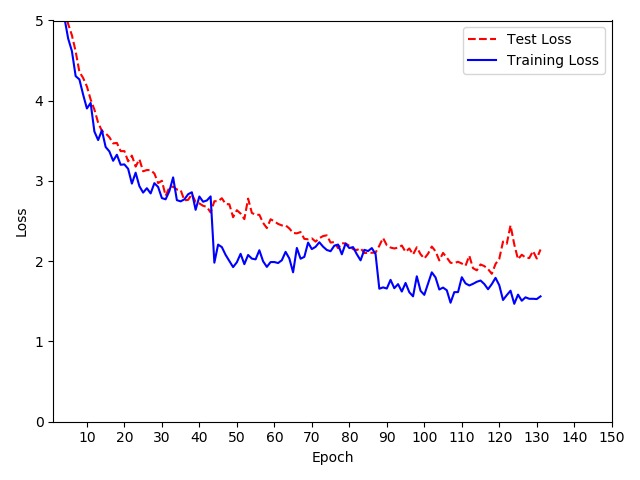
\includegraphics[width=8cm]{Bilder/ssdloss.jpeg} 
		\caption{Entwicklung der SSD Trainings- und Testverlustkurve während dem Training}
		\label{ssdloss}
	\end{center}
\end{figure}

Die Entscheidung zum \textit{Early Stopping} basiert auf dem Anstieg der Differenz zwischen Trainings- und Testverlustkurve ab Epoche 122, was auf \textit{Overfitting} schließen lässt. Zur Epoche davor war die Differenz der beiden Kurven am niedrigsten bei vergleichsweise geringem Verlust im Trainingsverfahren. Auffällig ist ebenfalls der große Abfall der Trainingsverlustkurve bei Epoche 45 und Epoche 89. Hier findet ein Wechsel im Kreuzvalidierungsverfahren statt. Die bessere Generalisierungsfähigkeit des Modells bei neuen Testdaten zeigt Ausschlag, indem die Klassifikationsergebnisse schlagartig besser werden und zu niedrigeren Kosten führen. Auch in Epoche 67 ist einer dieser Ausschläge zu sehen, der allerdings kleiner im Vergleich zu den anderen ausfällt. 

Zur Epoche 121 betrug das Ergebnis der Kostenfunktion 1.7. Es ergab eine \textit{mAP} von 83.1\%, leicht über den Referenzergebnissen von \textit{SSD} zu \textit{PascalVOC} (siehe Abbildung \ref{result}). Die Ergebnisse zu den einzelnen Klassen sind in folgender Tabelle dargestellt:

\begin{center}
	\begin{tabular}[H]{l|c}
		Klasse & mAP \\
		\hline
		Saskia Wasser Groß & 77.62\% \\
		Saskia Wasser Klein & 75.96\% \\
		Pepsi Cola Groß & 94.94\% \\
		Pepsi Cola Klein & 86.38\% \\
		ISO & 86.37\% \\
		ACE & 85.43\% \\
		Stenger Johannisbeerschorle & 69.47\% \\
		Stenger Apfelsaftschorle & 82.48 \% \\
		Vitamalz Malzbier & 76.24\%
	\end{tabular}
	\captionof{table}{Validierungsergebnisse SSD}
	\label{table:ssdresults}
\end{center}

Wird nun das trainierte Modell auf echte Daten angewendet, so fällt auf, dass manche Objekte doppelt detektiert werden. Um dieses Problem zu lösen, gibt es zwei Möglichkeiten. 

Als erstes kann bei der Detektion der minimale \textit{confidence score} angegeben werden, ab wann eine Detektion offiziell als solche wahrgenommen wird. Hier liegt die Herausforderung darin, einen optimalen Wert zu finden, sodass verdeckte Objekte noch als solche erkannt werden, aber doppelt erkannte Objekte nicht mehr auftreten. Der \textit{confidence score} wurde nach mehrmaligem Iterieren auf 0.7 festgelegt.

Die zweite Möglichkeit besteht darin, die maximale Überlappung zweier Bounding Boxen festzulegen. Somit werden doppelte Bounding Boxen, die sich flächenmäßig über einem gewissen Grenzwert überlappen, auf eine Bounding Box reduziert. Er stellte ich sich Parameter von 0.45 als geeignet heraus. Außerdem wurden Inkonsistenzen im Detektionsverhalten festgestellt.

\begin{figure}[H]
	\centering
	\subfigure[verdeckt]{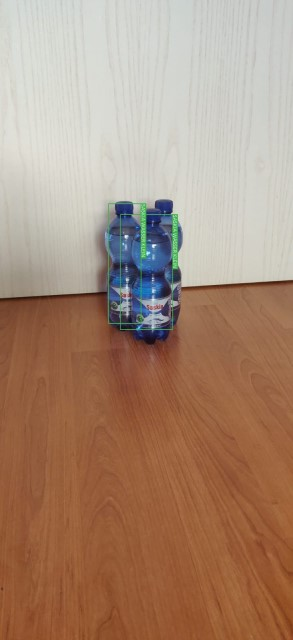
\includegraphics[width=0.30\textwidth]{Bilder/verdeckt.jpeg}}
	\hspace{2cm}
	\subfigure[winkel]{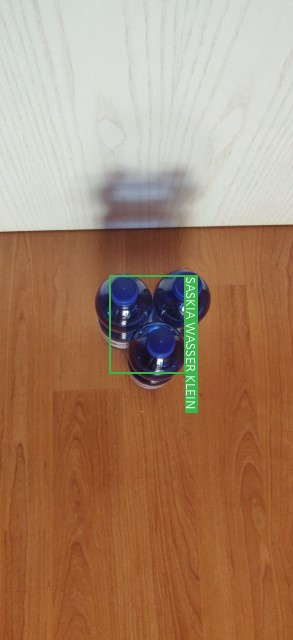
\includegraphics[width=0.30\textwidth]{Bilder/winkel.jpeg}}
	\caption{Detektionsverhalten von SSD bei extremen Blicklagen}
	\label{lagen}
\end{figure}

So sind von anderen Objekten verdeckte Objekte nur schwer zu erkennen, genauso wie Objekte aus extremen Blicklagen (siehe Abbildung \ref{lagen}). Diese Fälle wurden im Datensatz zwar zu 12.5\% abgedeckt, scheinen allerdings nur wenig Auswirkung auf besseres Detektionsverhalten für solche Fälle geliefert zu haben. Es lässt sich auch keine Aussage darüber treffen, ob eine Erweiterung des Datensatzes mit weiteren solchen Extremfällen eine Abhilfe für dieses Problem hätte liefern können. 

\begin{figure}[H]
	\subfigure[1 Meter]{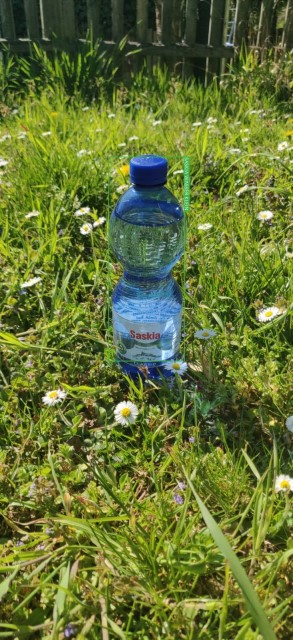
\includegraphics[width=0.30\textwidth]{Bilder/einmeter.jpeg}}\hfill
	\subfigure[2 Meter]{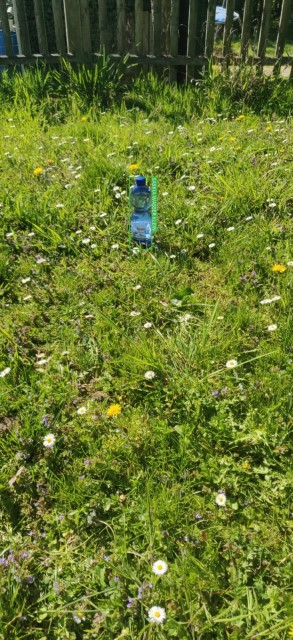
\includegraphics[width=0.30\textwidth]{Bilder/zweimeter.jpeg}}\hfill
	\subfigure[3 Meter]{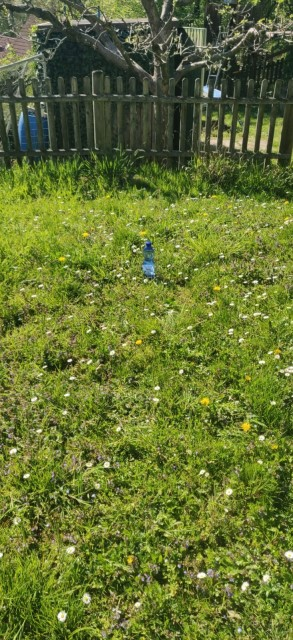
\includegraphics[width=0.30\textwidth]{Bilder/dreimeter.jpeg}}\hfill
	\caption{Detektionsverhalten von SSD bei unterschiedlichen Entfernungen}
	\label{entfernung}
\end{figure}

Auch die Entfernung zum zu detektierenden Objekt besitzt eine Auswirkung auf das Detektionsverhalten. In Abbildung \ref{entfernung} wird gezeigt, dass ab einer Entfernung von drei Metern keine Detektion mehr erfolgte. 

\begin{figure}[H]
	\subfigure[überbeleuchtet]{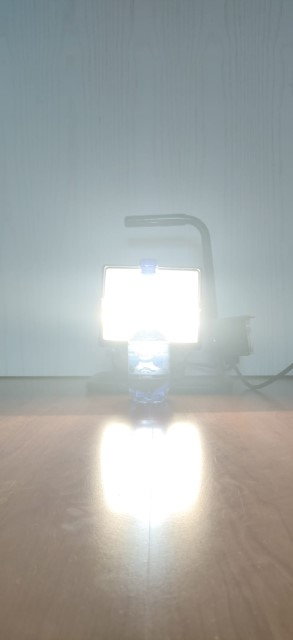
\includegraphics[width=0.30\textwidth]{Bilder/ueberbeleuchtet.jpeg}}\hfill
	\subfigure[normal]{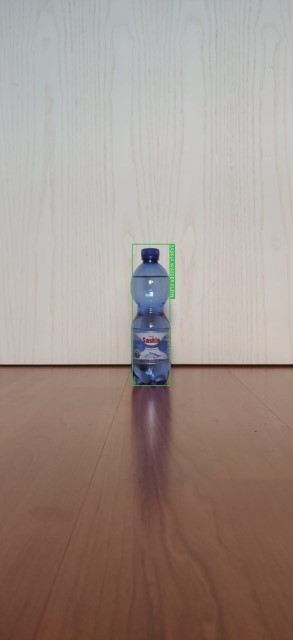
\includegraphics[width=0.30\textwidth]{Bilder/normalbeleuchtet.jpeg}}\hfill
	\subfigure[unterbeleuchtet]{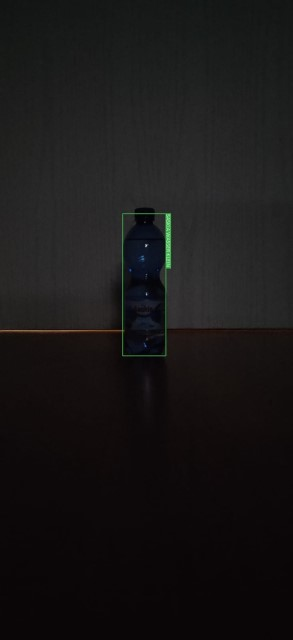
\includegraphics[width=0.30\textwidth]{Bilder/unterbeleuchtet.jpeg}}\hfill
	\caption{Detektionsverhalten von SSD bei unterschiedlichen Beleuchtungsverhältnissen}
	\label{sicht}
\end{figure}

Des Weiteren haben unterschiedliche Beleuchtungsgrade eine Auswirkung auf das Detektionsverhalten. In Abbildung \ref{sicht} wird unterschieden zwischen dem Detektionsverhalten bei überbeleuchteten, normalen und unterbeleuchteten Sichtverhältnissen. Überbeleuchtete Umgebungsverhältnisse erschweren die Objektdetektion in diesem Beispiel. 

Die Detektion reagierte allerdings invariant gegenüber unterschiedlichen Hintergründen oder Bildauflösungen.

\subsection*{YOLO}

Um eine möglichst gute Aussage über den Vergleich der beiden Objektdetektoren treffen zu können, kommt bei \textit{YOLO} der exakt gleiche Trainings- und Testdatensatz wie beim \textit{SSD} zum Einsatz. Das Training von \textit{YOLO} ergab eine \textit{mAP} von 80.36\%. Abbildung \ref{yolo_result} zeigt die Verbesserung des Modells während dem Trainingsprozess. 

\begin{figure}[H]
	\begin{center}
		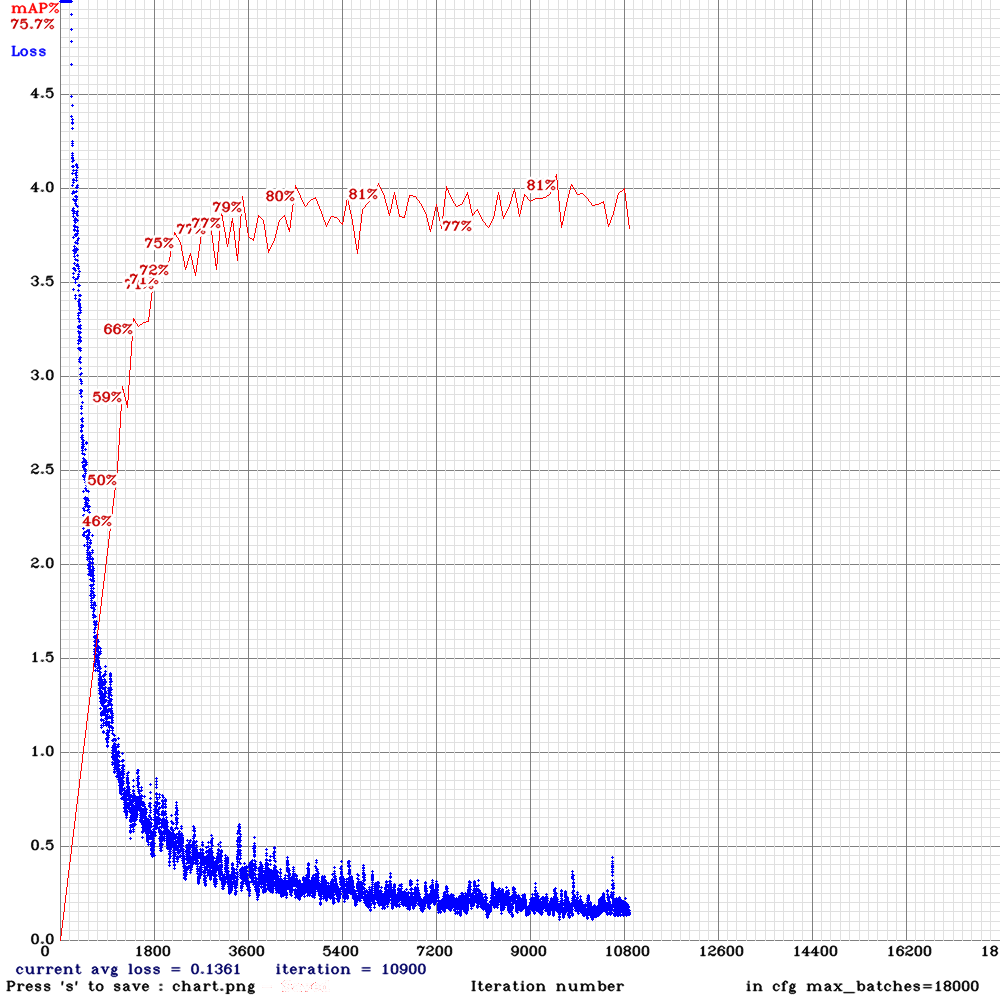
\includegraphics[width=8cm]{Bilder/yolo_result.png} 
		\caption{Entwicklung der YOLO Testverlustkurve und der \textit{mAP} während dem Training}
		\label{yolo_result}
	\end{center}
\end{figure}

Wie beim \textit{SSD} erreicht das Modell nach bereits etwa 4500 Batches eine \textit{mAP} von 80\%. Da sich das Modell ab diesem Zeitpunkt nicht mehr maßgeblich verbessert hat, wurde das Training vor Erreichung der durch die Dokumentation nahegelegte maximale Anzahl an Batches abgebrochen. Das frühe Erreichen eines sehr guten Ergebnis kann darauf zurückgeführt werden, dass es sich bei den gelabelten Klassen um Objekte des gleichen Typs handelt und das Modell dementsprechend leichter trainiert werden kann. 

Der \textit{confidence score} liegt standardmäßig bei 0.25. Nach mehreren Durchläufen stellt sich heraus, dass dieser Wert nicht verändert werden sollte. Ein zu geringer Wert sorgt zwar dafür, dass möglicherweise mehr Objekte erkannt werden, allerdings steigt damit auch die Rate an falsch oder doppelt erkannter Objekte. Ein Parameter für die Obergrenze der Überlappung zweier Bounding Boxen existiert nicht.

Tabelle \ref{table:yoloresults} zeigt die \textit{mAP} für jede Klasse.

\begin{center}
	\begin{tabular}[H]{l|c|c}
		Klasse & mAP & Differenz zu SSD\\
		\hline
		Saskia Wasser Groß & 76.69\% & (-0.93\%) \\
		Saskia Wasser Klein & 80.63\% & (+4.67\%) \\
		Pepsi Cola Groß & 73.14\% & (-21.8\%) \\
		Pepsi Cola Klein & 75.24\% & (-11.14\%) \\
		ISO & 90.28\% & (+3.91\%) \\
		ACE & 86.69\% & (+1.26\%) \\
		Stenger Johannisbeerschorle & 72.50\% & (+3.03\%) \\
		Stenger Apfelsaftschorle & 78.05\% & (-4.43\%) \\
		Vitamalz Malzbier & 81.94\% & (+5.7\%)
	\end{tabular}
	\captionof{table}{Validierungsergebnisse YOLO im Vergleich zu SSD}
	\label{table:yoloresults}
\end{center}

Auch bei \textit{YOLO} können verdeckte Objekte nur schwer erkannt werden. Ein Unterschied zu \textit{SSD} zeigt sich bei der Ansicht von oben:

\begin{figure}[H]
	\centering
	\subfigure[verdeckt]{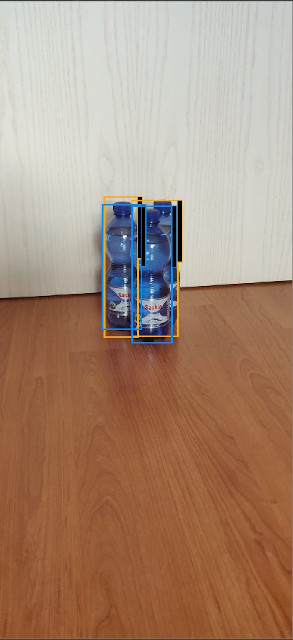
\includegraphics[width=0.30\textwidth]{Bilder/yolo_verdeckt.jpg}}
	\hspace{2cm}
	\subfigure[winkel]{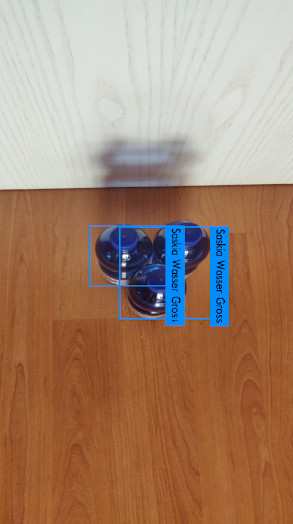
\includegraphics[width=0.30\textwidth]{Bilder/yolo_winkel.jpg}}
	\caption{Detektionsverhalten von YOLO bei extremen Blicklagen}
	\label{lagen_yolo}
\end{figure}

Hier werden zwei von drei Flaschen erkannt, die allerdings der falschen Klasse (\textit{Saskia Wasser Groß} statt \textit{Saskia Wasser Klein}) zugeordnet werden und eine der zwei Bounding Boxes zwei Flaschen umschließt.

\begin{figure}[H]
	\subfigure[1 Meter]{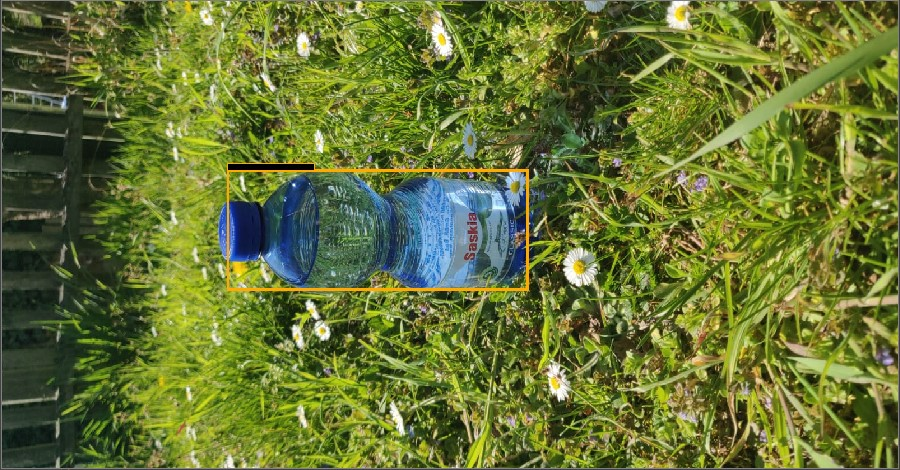
\includegraphics[width=0.30\textwidth]{Bilder/yolo_entfernung1.jpg}}\hfill
	\subfigure[2 Meter]{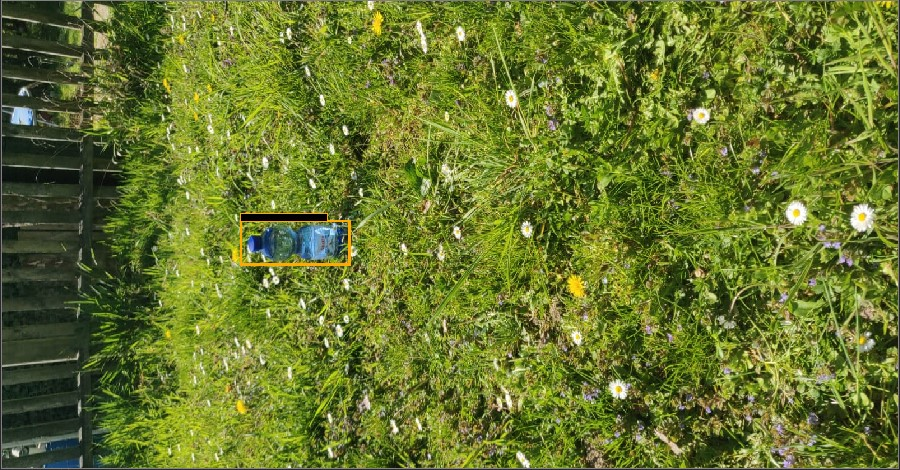
\includegraphics[width=0.30\textwidth]{Bilder/yolo_entfernung2.jpg}}\hfill
	\subfigure[3 Meter]{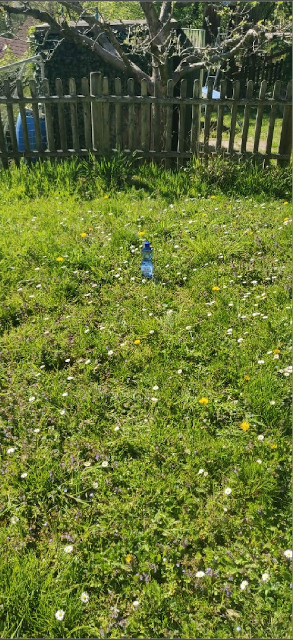
\includegraphics[width=0.30\textwidth]{Bilder/yolo_entfernung3.jpg}}\hfill
	\caption{Detektionsverhalten von YOLO bei unterschiedlichen Entfernungen}
	\label{entfernung_yolo}
\end{figure}

Wie bei \textit{SSD} erfolgt nach bereits drei Metern Entfernung keine Detektion mehr (siehe Abbildung \ref{entfernung_yolo}). Der \textit{confidence score} für die korrekt erkannte Bounding Box liegt bei nur 2\%.
 
\begin{figure}[H]
 	\subfigure[überbeleuchtet]{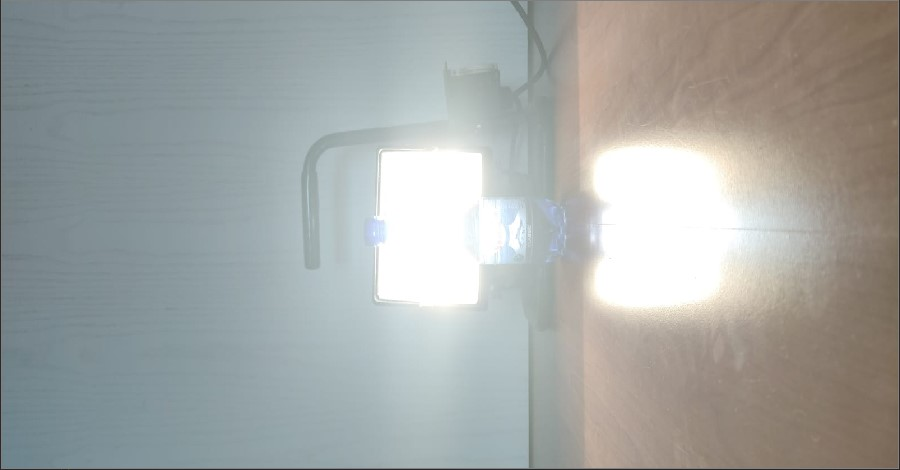
\includegraphics[width=0.30\textwidth]{Bilder/yolo_beleuchtung2.jpg}}\hfill
 	\subfigure[normal]{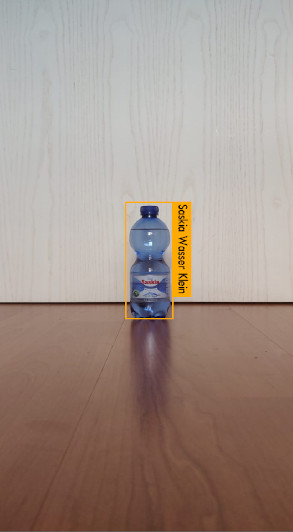
\includegraphics[width=0.30\textwidth]{Bilder/yolo_beleuchtung1.jpg}}\hfill
 	\subfigure[unterbeleuchtet]{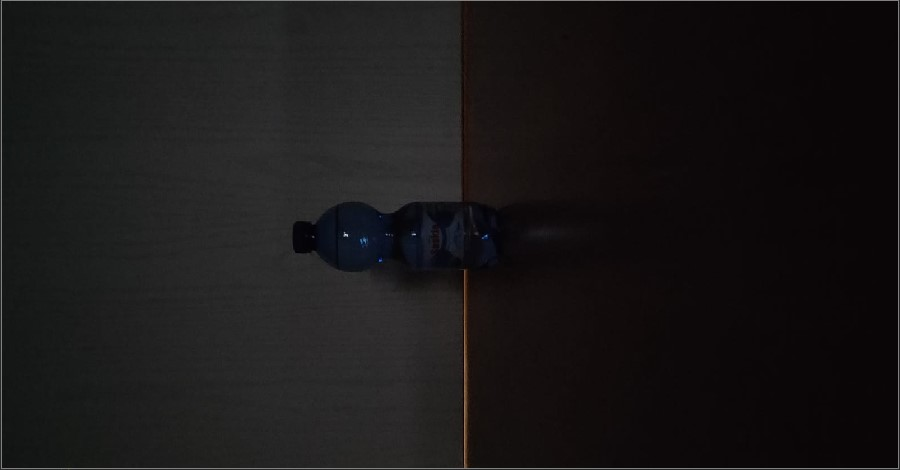
\includegraphics[width=0.30\textwidth]{Bilder/yolo_beleuchtung3.jpg}}\hfill
 	\caption{Detektionsverhalten von YOLO bei unterschiedlichen Beleuchtungsverhältnissen}
 	\label{sicht_yolo}
\end{figure}

Beim Testen der verschiedenen Beleuchtungsverhältnisse fällt auf, dass im Gegensatz zum \textit{SSD} die Flasche in der unterbelichteten Umgebung nicht erkannt wird beziehungsweise mit einem \textit{confidence score} von nur 6\%. 

Gleich zu \textit{SSD} reagiert \textit{YOLO} auch invariant gegenüber unterschiedlichen Hintergründen oder Bildauflösungen.
 
\section{Reaktionsvermögen}

Bei der Inferenz fällt allerdings entgegen der Erwartungen auf, dass die Inferenz überdurchschnittlich langsam verläuft. Das Problem lässt sich auf die synchrone Arbeitsweise der bisherigen Detektionsalgorithmen zurück führen, bei dem erst ein neuer Frame des Videostreams angefragt wird, sobald das aktuelle Bild durch die Vorverarbeitung gelaufen ist und durch das Modell inferiert wurde. 

Um dem entgegen zu wirken, wurde ein Bufferkonzept in einem parallelem Thread realisiert, der einzelne Frames zeitgleich zur Inferenz anfragt und zwischenspeichert. Ist der Buffer voll, so werden nach dem \textit{First In First Out} Verfahren die älteren Frames verworfen. Dadurch konnte die FPS Anzahl von \textit{SSD} von maximal 18 auf die vollen 30 und bei \textit{YOLO} von 20 auf 28 gesteigert werden. Dadurch sollten sämtliche Änderungen in der Umgebung rechtzeitig vom Objektdetektor erkannt werden. 

Ein weiteres Problem beschreibt die initiale Latenz zwischen der Inferenz und der Bildaufnahme. Die Inferenz kann erst gestartet werden, sobald die Gewichtungen des Modells initialisiert und geladen wurden. Bei \textit{YOLO} benötigt die Initialisierung etwa drei Sekunden, bei \textit{SSD} vier Sekunden. Das lässt sich umgehen, indem entweder der Thread zur Bildaufnahme verzögern gestartet wird oder dessen Buffer kleiner gewählt wird.

\section{Trainingsverhalten}

\begin{center}
	\begin{tabular}[H]{l|c|c|c|c}
		Detektor & Hardware & Batch Größe & Dauer Epoche & Dauer Insgesamt \\
		\hline
		SSD & GTX 1080 & 16 & 9 Min. & 16.5 Std. \\
		YOLO & RTX 2060 & 64 & 1.5 Min. & 8 Std.
	\end{tabular}
	\captionof{table}{Trainingsverhalten von SSD und YOLO}
	\label{table:duration}
\end{center}

Tabelle \ref{table:duration} zeigt die Ergebnisse des Trainingsverhaltens von \textit{SSD} und \textit{YOLO}. Pro Epoche wurden 998 Bilder durchlaufen. Die Dauer der beiden Trainingsdurchläufe lässt sich allerdings nur schwer vergleichen. Zum einen wird für das Training von \textit{YOLO} eine andere GPU verwendet, deren Tensor Kerne den Trainingsprozess merklich beschleunigen. Zum anderen werden die beiden Objektdetektoren in zwei verschiedenen Frameworks implementiert, wodurch ein anderes Trainingsverhalten von Grund auf gegeben ist und Unterschiede in der Performance auftreten können. Auch die Batch Größe wurde unterschiedlich gewählt, was sich auf die Häufigkeit des Gradientenabstiegs auswirkt. Bei beiden Verfahren kann das Training durch die Ablage von sogenannten Modell-Checkpoints zu einem späteren Zeitpunkt fortgeführt werden. Das ist vor allem dann von Vorteil, wenn nachträglich Parameter oder Trainingsdaten angepasst werden und kein kompletter Neustart des Trainings erforderlich ist.


\chapter{Bewertung}

\begin{itemize}
	\item Ergebnisse bewerten und diskutieren
	\item Was liefert die Arbeit, was bisher noch nicht bekannt war (Mehrwert, auch wenn etwas nicht geht)?
\end{itemize}


\chapter{Zusammenfassung und Ausblick}

Ziel der Arbeit war es zum einen zu evaluieren, wie gut die bestehenden Objektdetektoren für industrielle Anwendungsszenarien grundsätzlich geeignet sind, zum anderen, ob das spezifische Anwendungsszenario zur Durchführung einer Inventur von Warenhäusern mit einer Drohne prototypisch umsetzbar ist. Nach dieser Arbeit sind nun folgende Erkenntnisse festzuhalten.

Zunächst ist evaluiert worden, dass Objektdetektoren wie \textit{SSD} und \textit{YOLO} durchaus das Potential ausweisen, industriell genutzt zu werden. Nicht nur hinsichtlich ihrer Präzision im Detektionsvermögen weisen sie zuversichtliche Ergebnisse auf, sondern auch in der Schnelligkeit ihrer Detektion. Beide weisen bei speziellen Detektionsszenarien ihre Stärken und Schwächen auf. Gerade die Detektion von teilweise verdeckten Objekten stellt nach wie vor ein Problem dar, für das alternative Lösungswege gefunden werden müssen. 

Daneben stellt sich die Machbarkeitsstudie \textit{Smart Warehouse} basierend auf den gegebenen Rahmenbedingungen und den getroffenen Entscheidungen als nicht machbar heraus. Es wurde eine Drohne programmiert, die ein Miniaturmodell eines Warenhauses durchfliegt. Ihr Drohnenstream konnte zwar abgefragt werden, allerdings wegen Kompatibilitätsproblemen der Laufzeitumgebungen nicht durch ein \textit{Deep Learning} Modell inferiert werden. Anstelle eines Video-Streams der Drohne wurde ein Video-Stream einer Webcam an einen Server zur Inferenz mit dem \textit{YOLO} Objektdetektionsmodell gesendet und die daraus resultierenden Objekte gezählt. Das Ergebnis und der Live-Stream der Inferenz wurden auf einer Webapplikation dargestellt. Offen bleibt das Problem einer doppelten Detektion von Objekten bei mehrfachen Erscheinen im Bild nach gewissen zeitlichen Abständen, da keine eindeutige Identifizierung von Objekten mit reiner Objektdetektion möglich ist. Damit wäre das Zählen von gleichen Objekten an unterschiedlichen Lagerplätzen mit Hilfe eines Objektdetektors nicht umsetzbar, zumindest nicht ohne weitere Zuhilfenahme von zum Beispiel einem GPS Sensor. Auch das Detektieren von verdeckten Objekten bleibt eine weitere Problematik.

Um das \textit{Smart Warehouse} Szenario weiter auszubauen, soll als nächstes der Datensatz vom simplen Beispiel von Getränkeflaschen auf eine echte Warenhausumgebung erweitert werden. Dadurch wird ebenfalls erhofft, die Präzision des Modells weiter zu verbessern und Inkonsistenzen bei unterschiedlichen Beleuchtungsverhältnissen, extremen Blicklagen, größeren Entfernungen und unterschiedlichen Verdeckungsgraden zu beheben. Zudem muss die Flugsequenz der Drohne dahingehend optimiert werden, bei Stellen starker Verdeckungsgrade alternative Betrachtungswinkel zu wählen. 

Als nächstes muss ein eigener H.264 Decoder implementiert werden, der die neuste Python Version unterstützt und im Einklang mit den verwendeten \textit{Deep Learning} Frameworks steht. Nach diesem Schritt könnten anschließend auch Live-Bilder des Video-Streams der Drohne inferiert werden.

Um abschließend spezielle Rahmenbedingungen bei der Zählung durch Objektdetektion auszuschließen, könnte das Szenario ebenso zur eindeutigen Identifizierung von Objekten mit konventionellen RFID Chips erweitert werden. Dies ermöglicht ebenso neue Szenarien zu entwickeln, in denen Objektdetektion nur Suche von Objekten einer bestimmten Klasse genutzt wird und deren Identität anschließend mit RFID Chips sichergestellt wird. 

Bei Berücksichtigung dieser Verbesserungsvorschläge, lässt sich somit durchaus auf eine Umsetzbarkeit des \textit{Smart Warehouse} Szenarios in der Zukunft hoffen.


% ---- Literaturverzeichnis
\cleardoublepage
\renewcommand*{\chapterpagestyle}{plain}
\pagestyle{plain}
\pagenumbering{Roman}                   % Römische Seitenzahlen
\setcounter{page}{\numexpr\value{savepage}+1}

\printbibliography[title=Literaturverzeichnis]
%\chapter*{Literaturverzeichnis}
%\addcontentsline{toc}{chapter}{Literaturverzeichnis}
%\printbibheading 
%\printbibliography[keyword=book,heading=subbibliography,title={Literaturquellen}] % Ausgabe der Literaturquellen
%\printbibliography[keyword=online,heading=subbibliography,title={Internetquellen}]     % Ausgabe der Internetquellen

% ---- Anhang

\newgeometry{
	left=2.5cm,
	right=2.5cm,
	top=0cm,
	bottom=2.5cm,
	includeheadfoot
}

\appendix
\chapter{Anhang}
%\captionsetup{list=false}

\section*{Abbildungen}



\restoregeometry
\newpage

\onehalfspacing
%\include{Inhalt/12_Anhang/...}

%\clearpage
%\pagenumbering{Roman}  % römische Seitenzahlen für Anhang

\end{document}
